\section{Scenes and Focal Lengths}
\seclabel{sceneFocal}
The focal length of a camera defines its field of view and hence determines how much of a scene is captured in an image taken by the camera. It is an important calibration parameter for obtaining metric, as opposed to projective, measurements from images. It is usually calibrated using multiple images of a known object \cite{zhang2000flexible}, such as a chessboard, or as part of bundle adjustment \cite{triggs2000bundle}, from multiple images of realistic scenes. Well known existing approaches require a minimum set of vanishing lines  \cite{wang1991camera} or exploit Manhattan-world assumptions \cite{caprile1990using}. These techniques are very precise and elegant, but not generally applicable (e.g. beach or forest images, etc.).

We propose instead a learning approach that predicts focal length based on statistical dependencies between scene classes and fields of view. Given the same scene, images taken with large focal lengths will have fewer things in them than those captured with small focal lengths and this provides a cue for determining focal length. However certain scenes also have more things than others. This ambiguity can be resolved by training a predictor with many images of each scene class, taken with different focal lengths. 

Additionally, certain scenes tend to be pictured with preferred focal lengths. As an example, consider a scene class of ``pulpits". If a picture of a pulpit is taken with a short focal length, then the whole church will be visible and that image will not be tagged as a pulpit scene. In order for a pulpit to be dominant in a picture taken with a short focal length camera, then the photographer would have to be unnaturally close to it. 

\paragraph{Data:} We use the Places database \cite{zhou2014learning}, a large dataset that provides a dense sampling of scenes in natural images: it has $205$ scene classes, as diverse as \textit{swimming pool} and \textit{rope bridge}, and $2.5$ million images. We were able to scrape focal length metadata from EXIF tags of approximately $20$k examples, on average 100 per class, and split these into a training set having $15$k and a validation set of $5$k images. 

\paragraph{Learning:} We considered the problem of predicting the ratio of the focal length to the camera sensor width, which when multiplied by the size of the image in pixels gives the desired the focal length in pixels. We clustered the logarithm of this ratio into $10$ bins using k-means and formulated the prediction problem as classification, using a softmax loss. Images in the bin with highest and smallest focal length ratio are shown in \figref{focal_lengths}. We experimented finetuning different popular convolutional networks, including two trained on Imagenet classification -- AlexNet \cite{krizhevsky2012imagenet} and VGG-Deep16 \cite{simonyan2014very} -- and a network trained on the Places scenes -- the PlacesNet \cite{zhou2014learning}.

\begin{figure}[htb!]
  \centering
  \includegraphics[width=0.32\textwidth]{figures/amodal/highest4}
  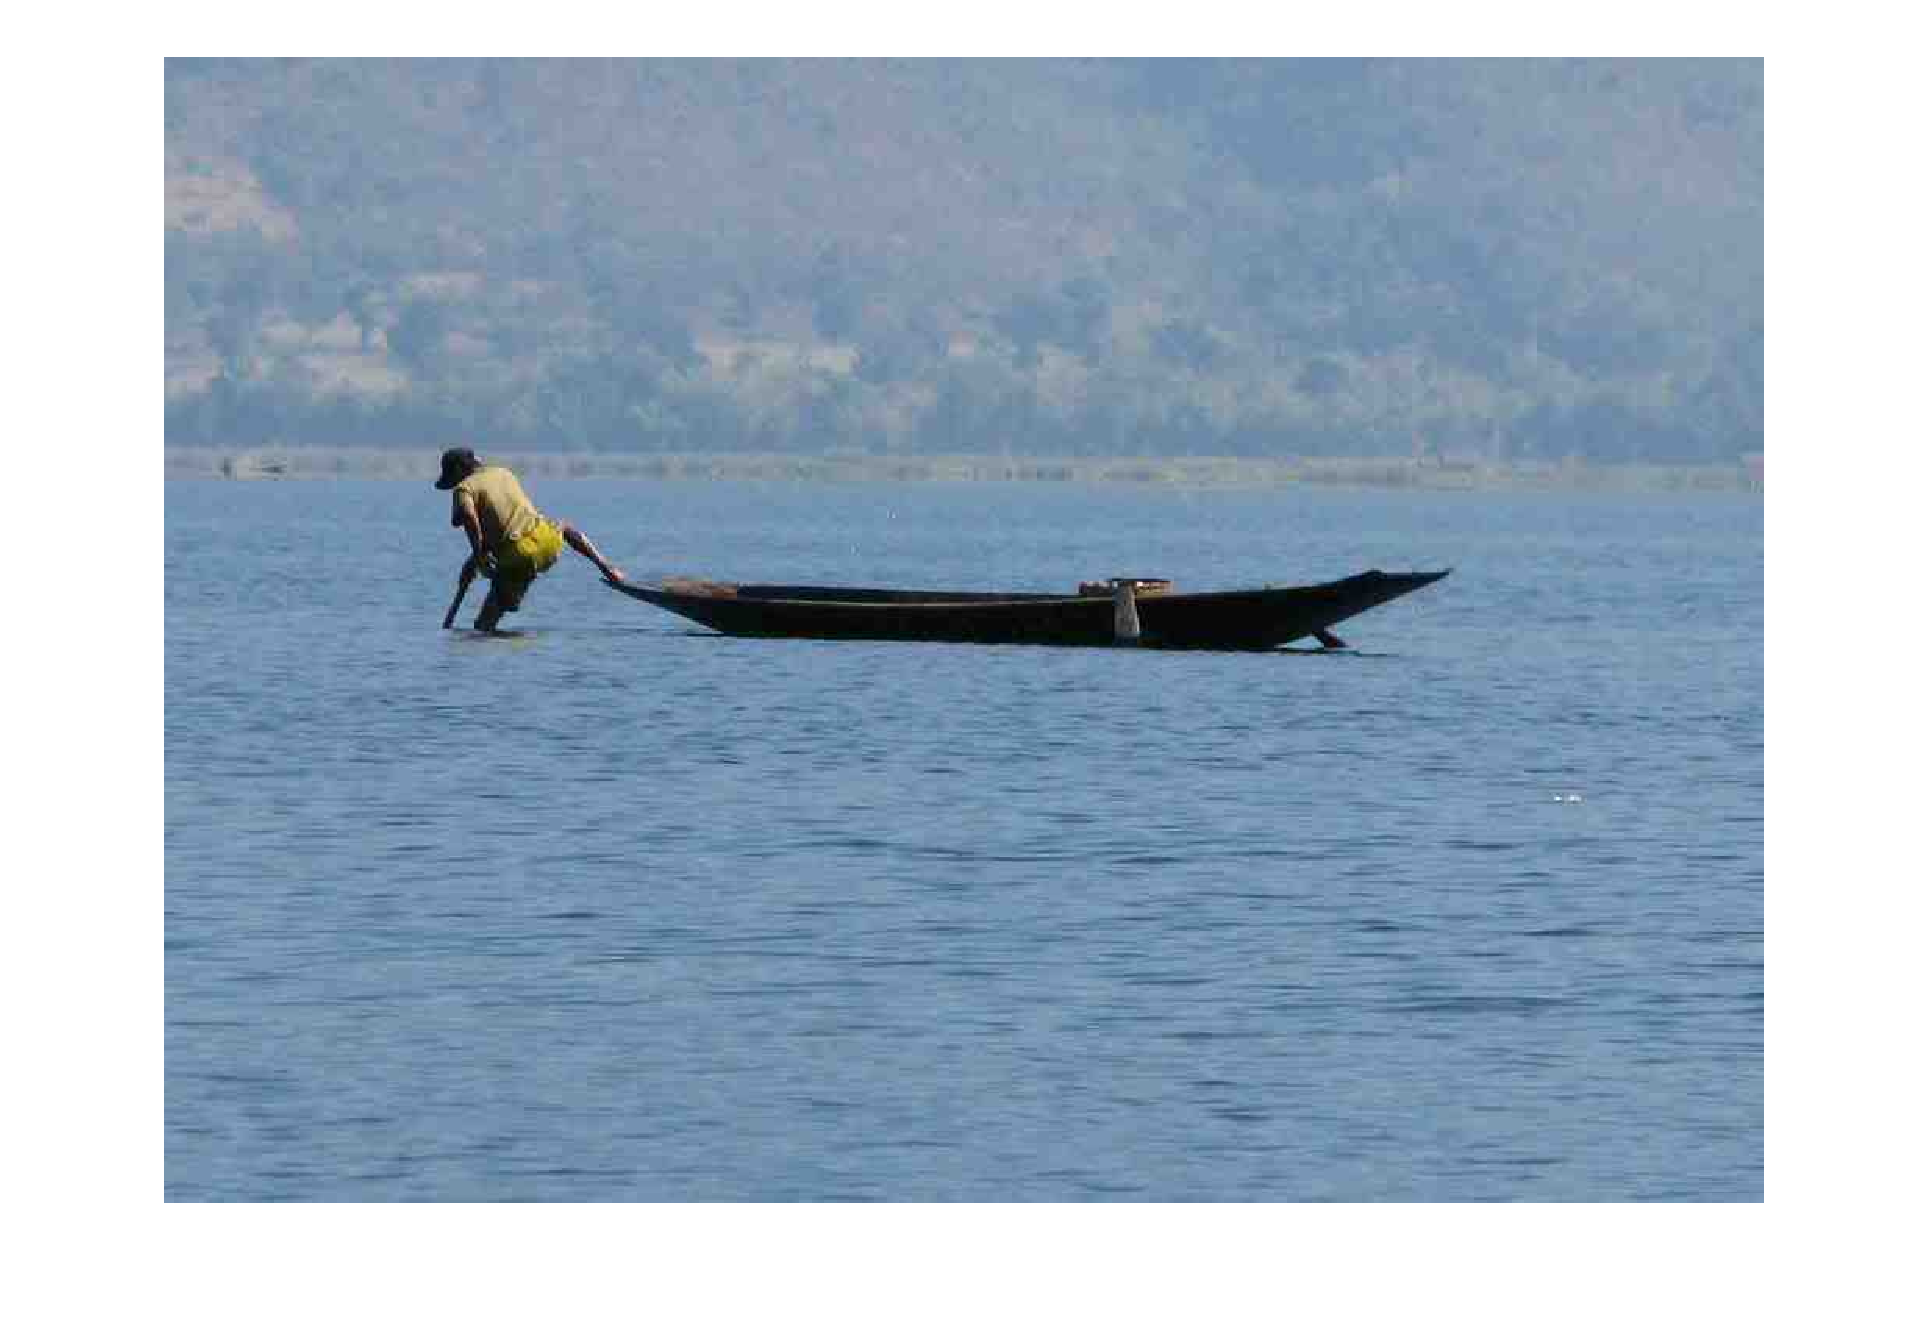
\includegraphics[width=0.32\textwidth]{figures/amodal/highest3}  
  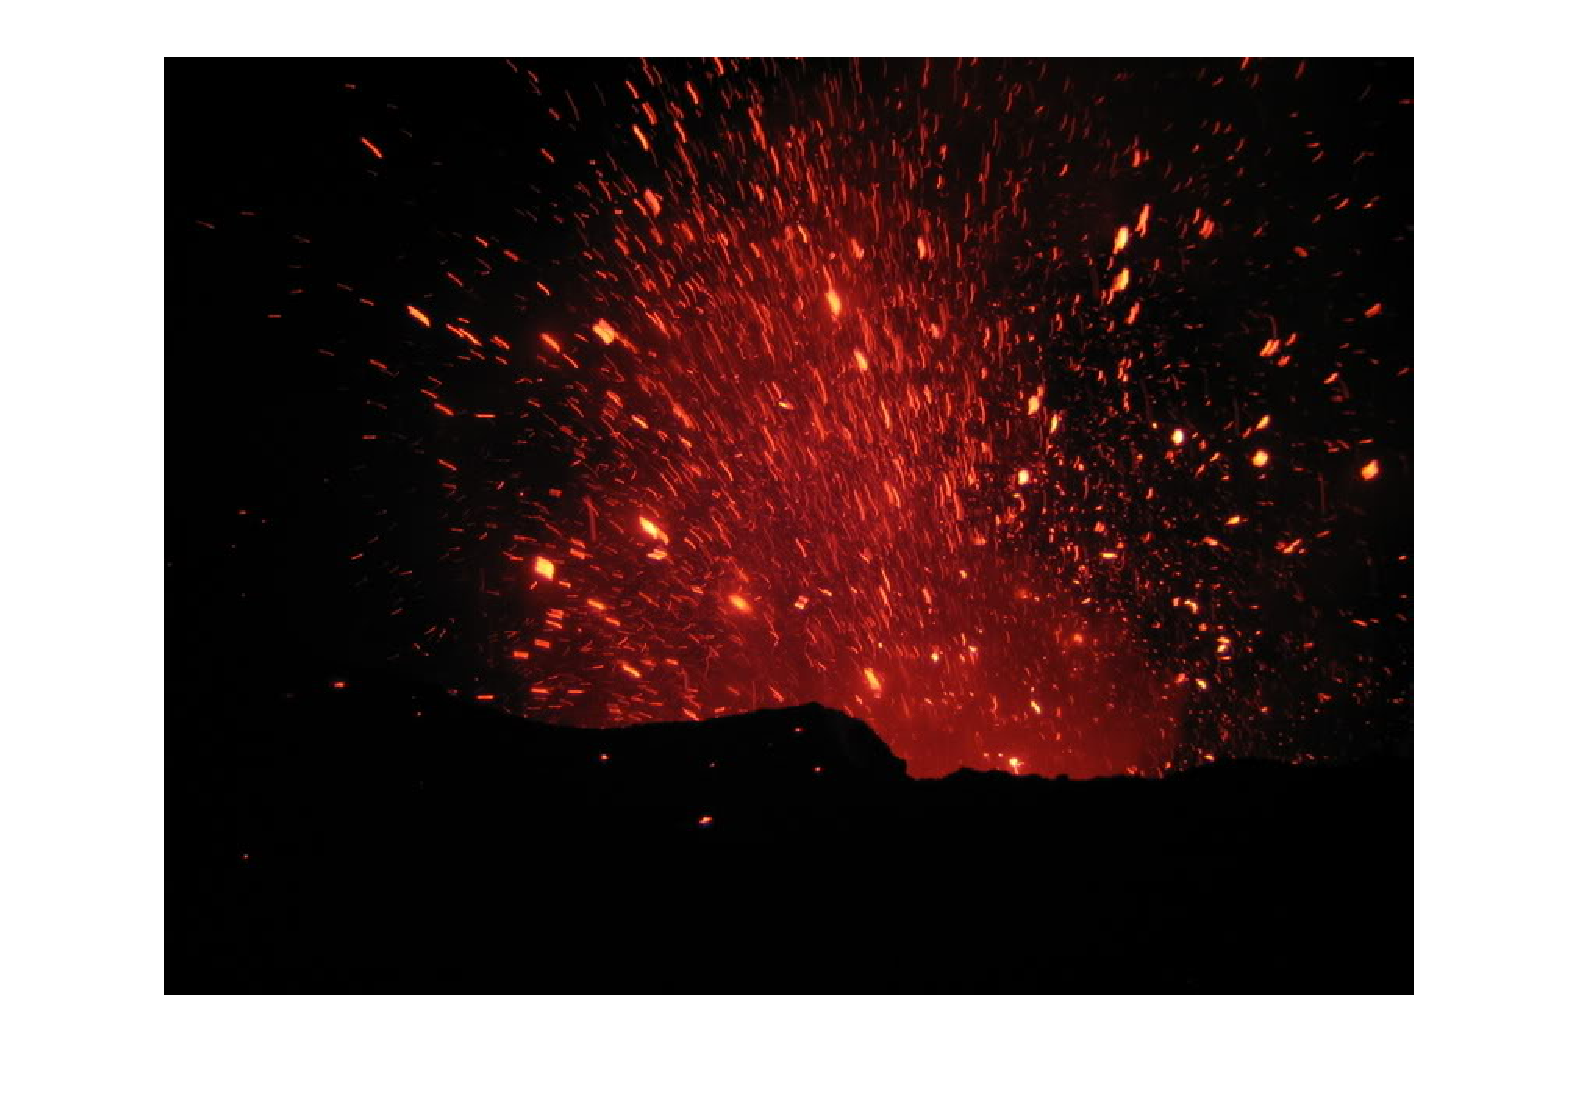
\includegraphics[width=0.32\textwidth]{figures/amodal/highest6}  
  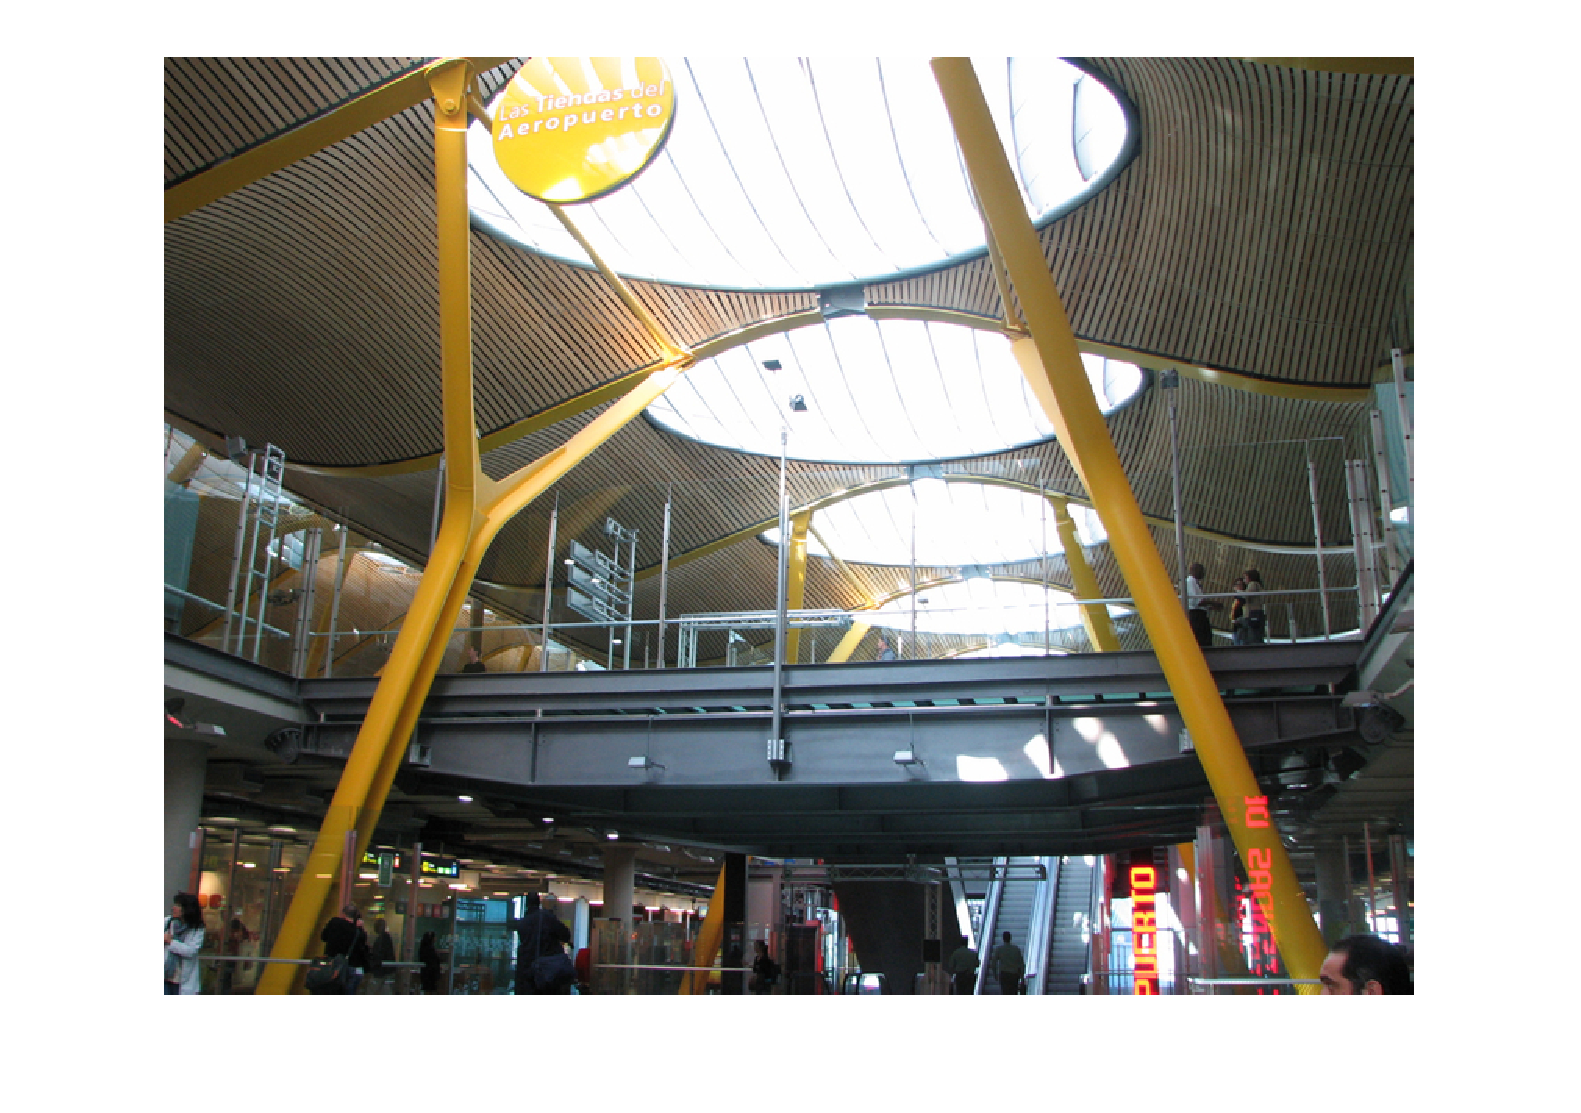
\includegraphics[width=0.32\textwidth]{figures/amodal/lowest1}
  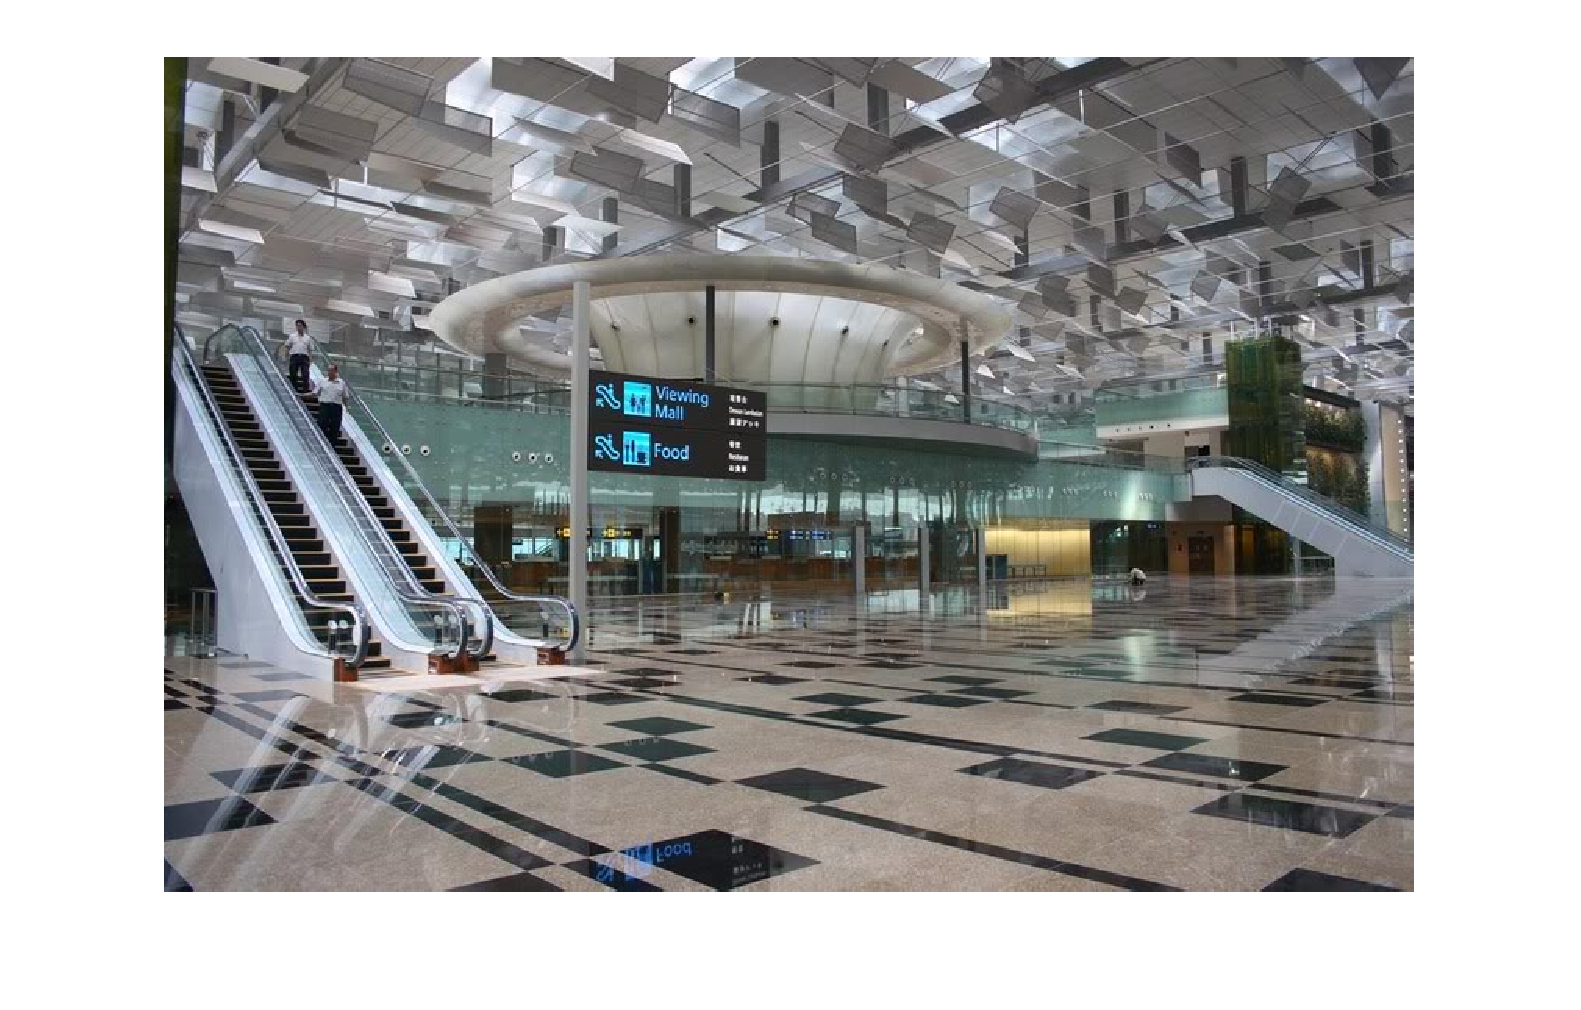
\includegraphics[width=0.32\textwidth]{figures/amodal/lowest3}  
  \includegraphics[width=0.32\textwidth]{figures/amodal/lowest7}
  \caption{\figlabel{focal_lengths} Example images from the Places dataset from clusters with the largest (up) and smallest (down) focal lengths. Note how images with small focal lengths tend to be more cluttered. A pattern we observed is that dangerous or unaccessible scenes, such as those having volcanos, wild animals and boats tend to be captured using very-high focal lengths,  which is rational.}
\end{figure}

\begin{figure}[htb!]
  \centering
  \begin{minipage}{.45\textwidth}
    \centering
    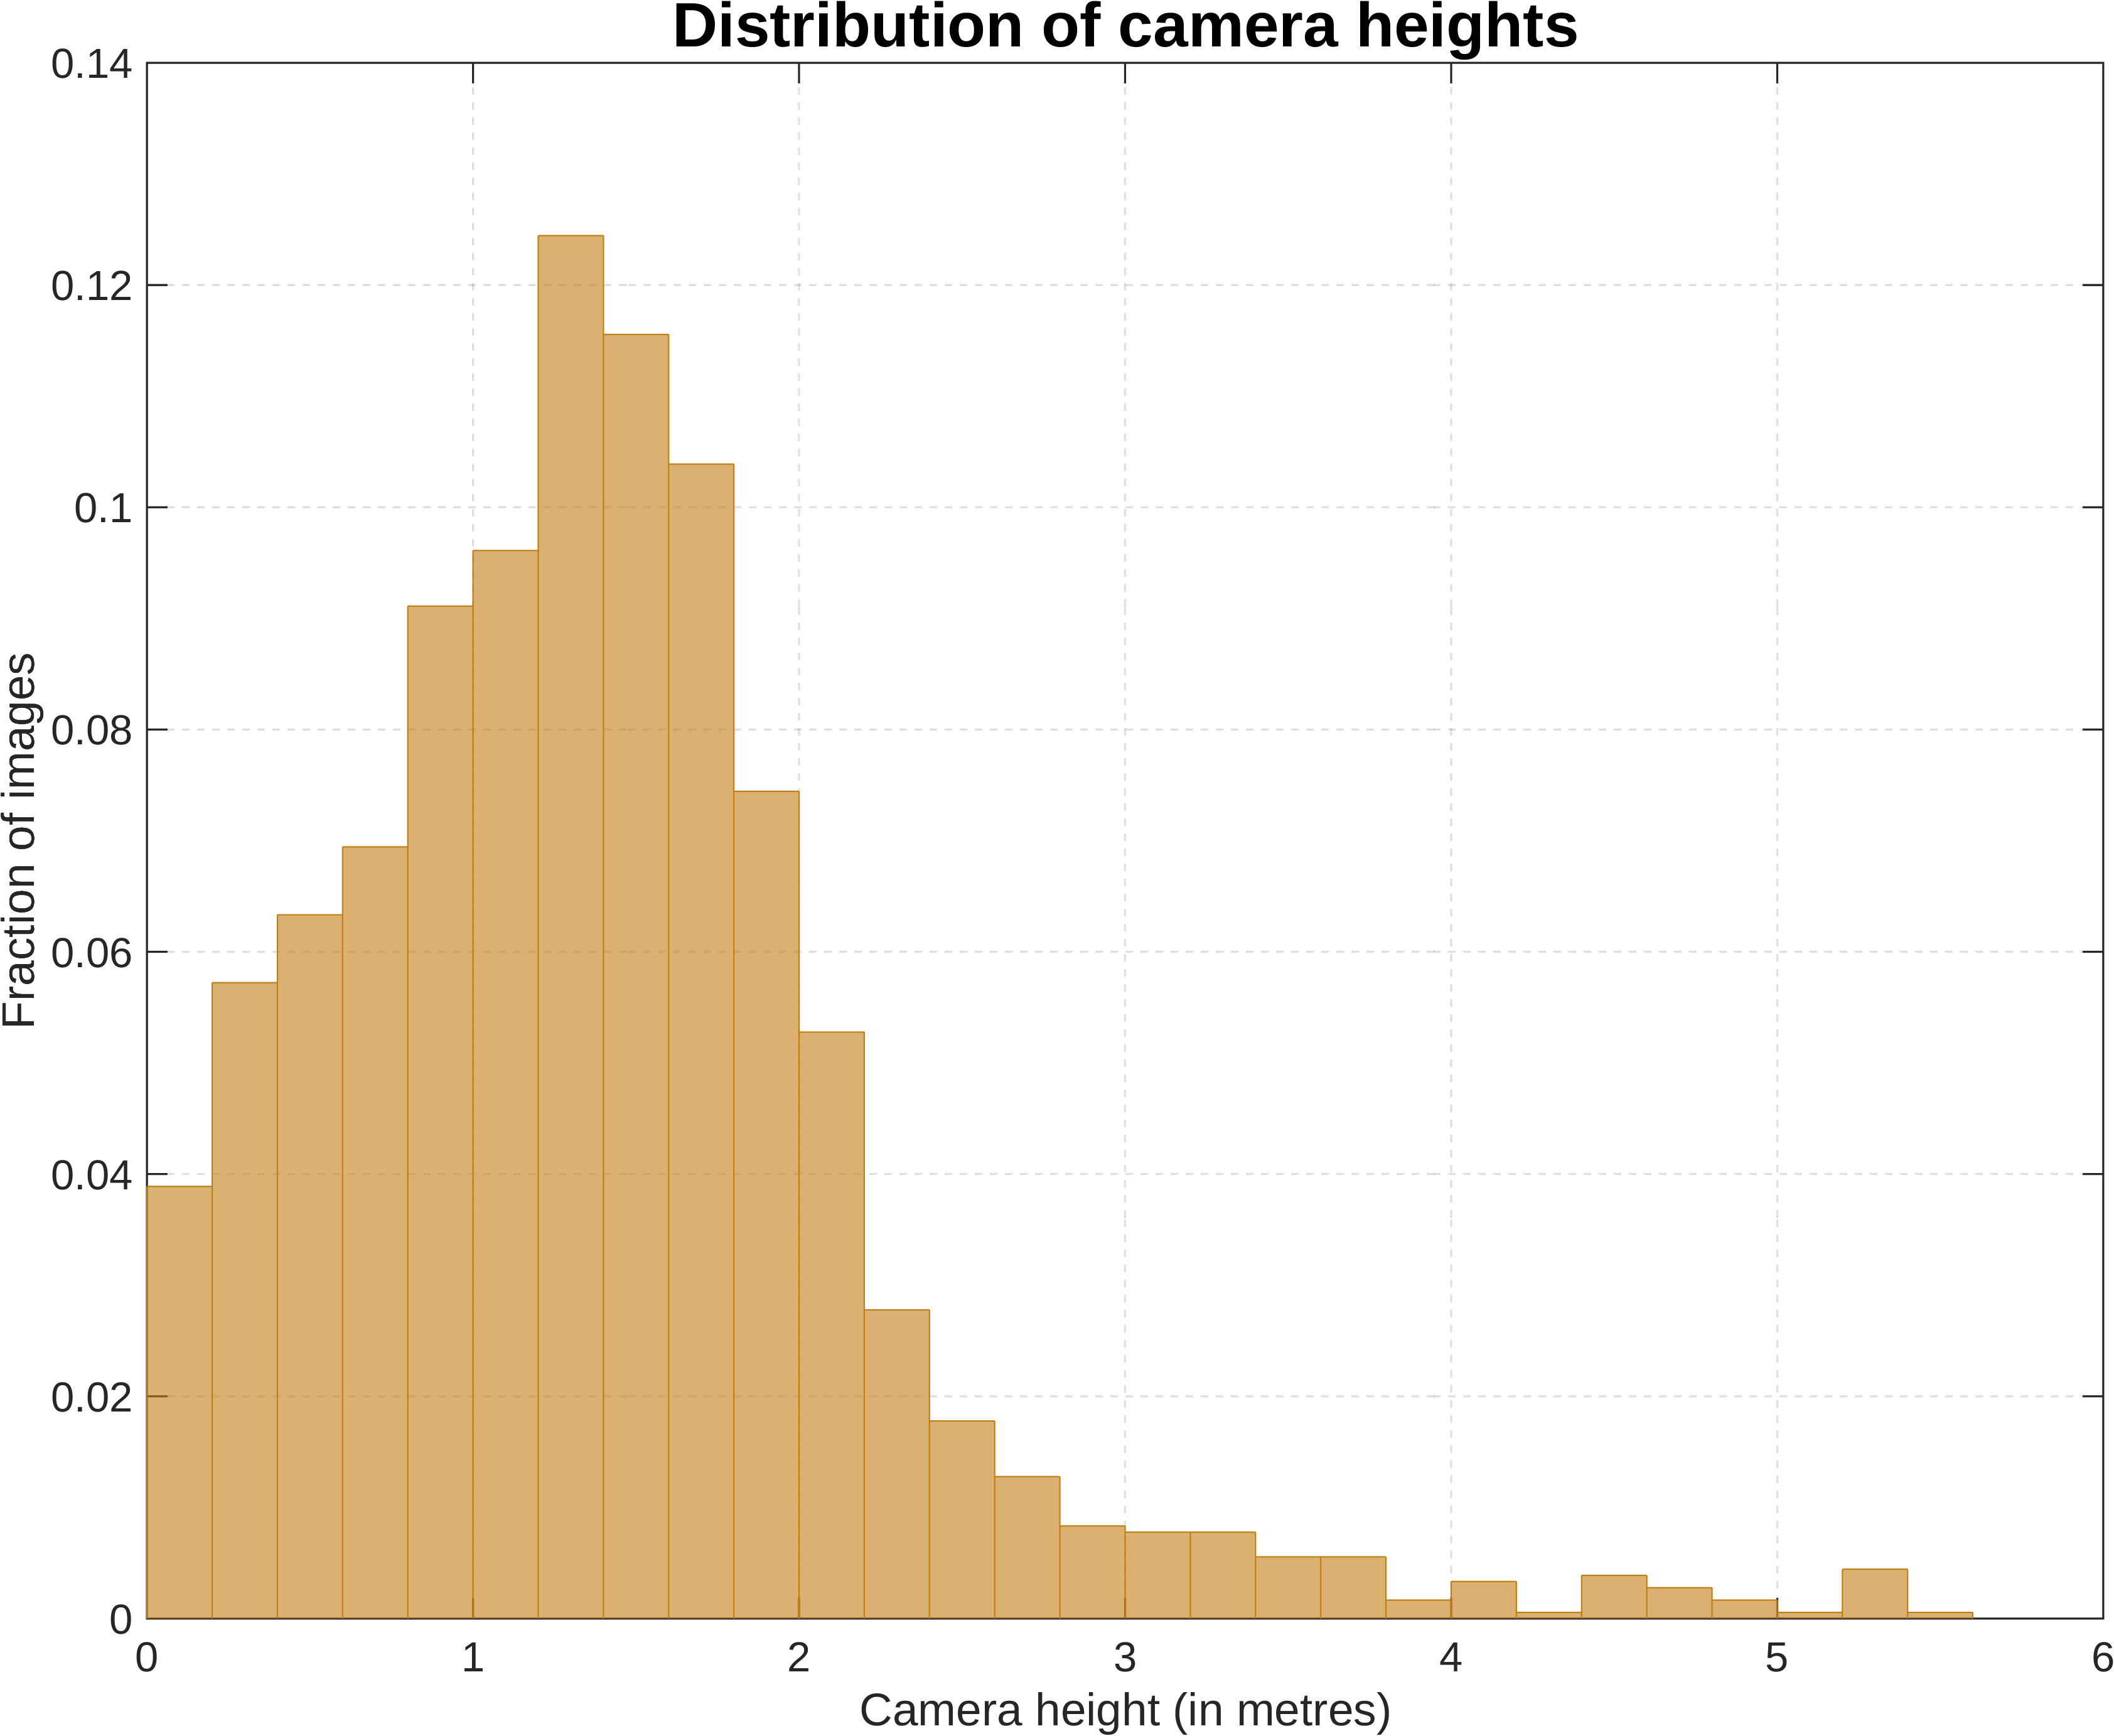
\includegraphics[width=0.95\linewidth]{figures/amodal/heights_pred_choc.png}
    \caption{\figlabel{heightDistr} Distribution of camera heights as inferred on PASCAL VOC. It can be seen that the distribution is peaked around the height at which humans normally take pictures (1.4m) with a long tail.}
  \end{minipage}
  \hfill
  \begin{minipage}{.45\textwidth}
    \centering
    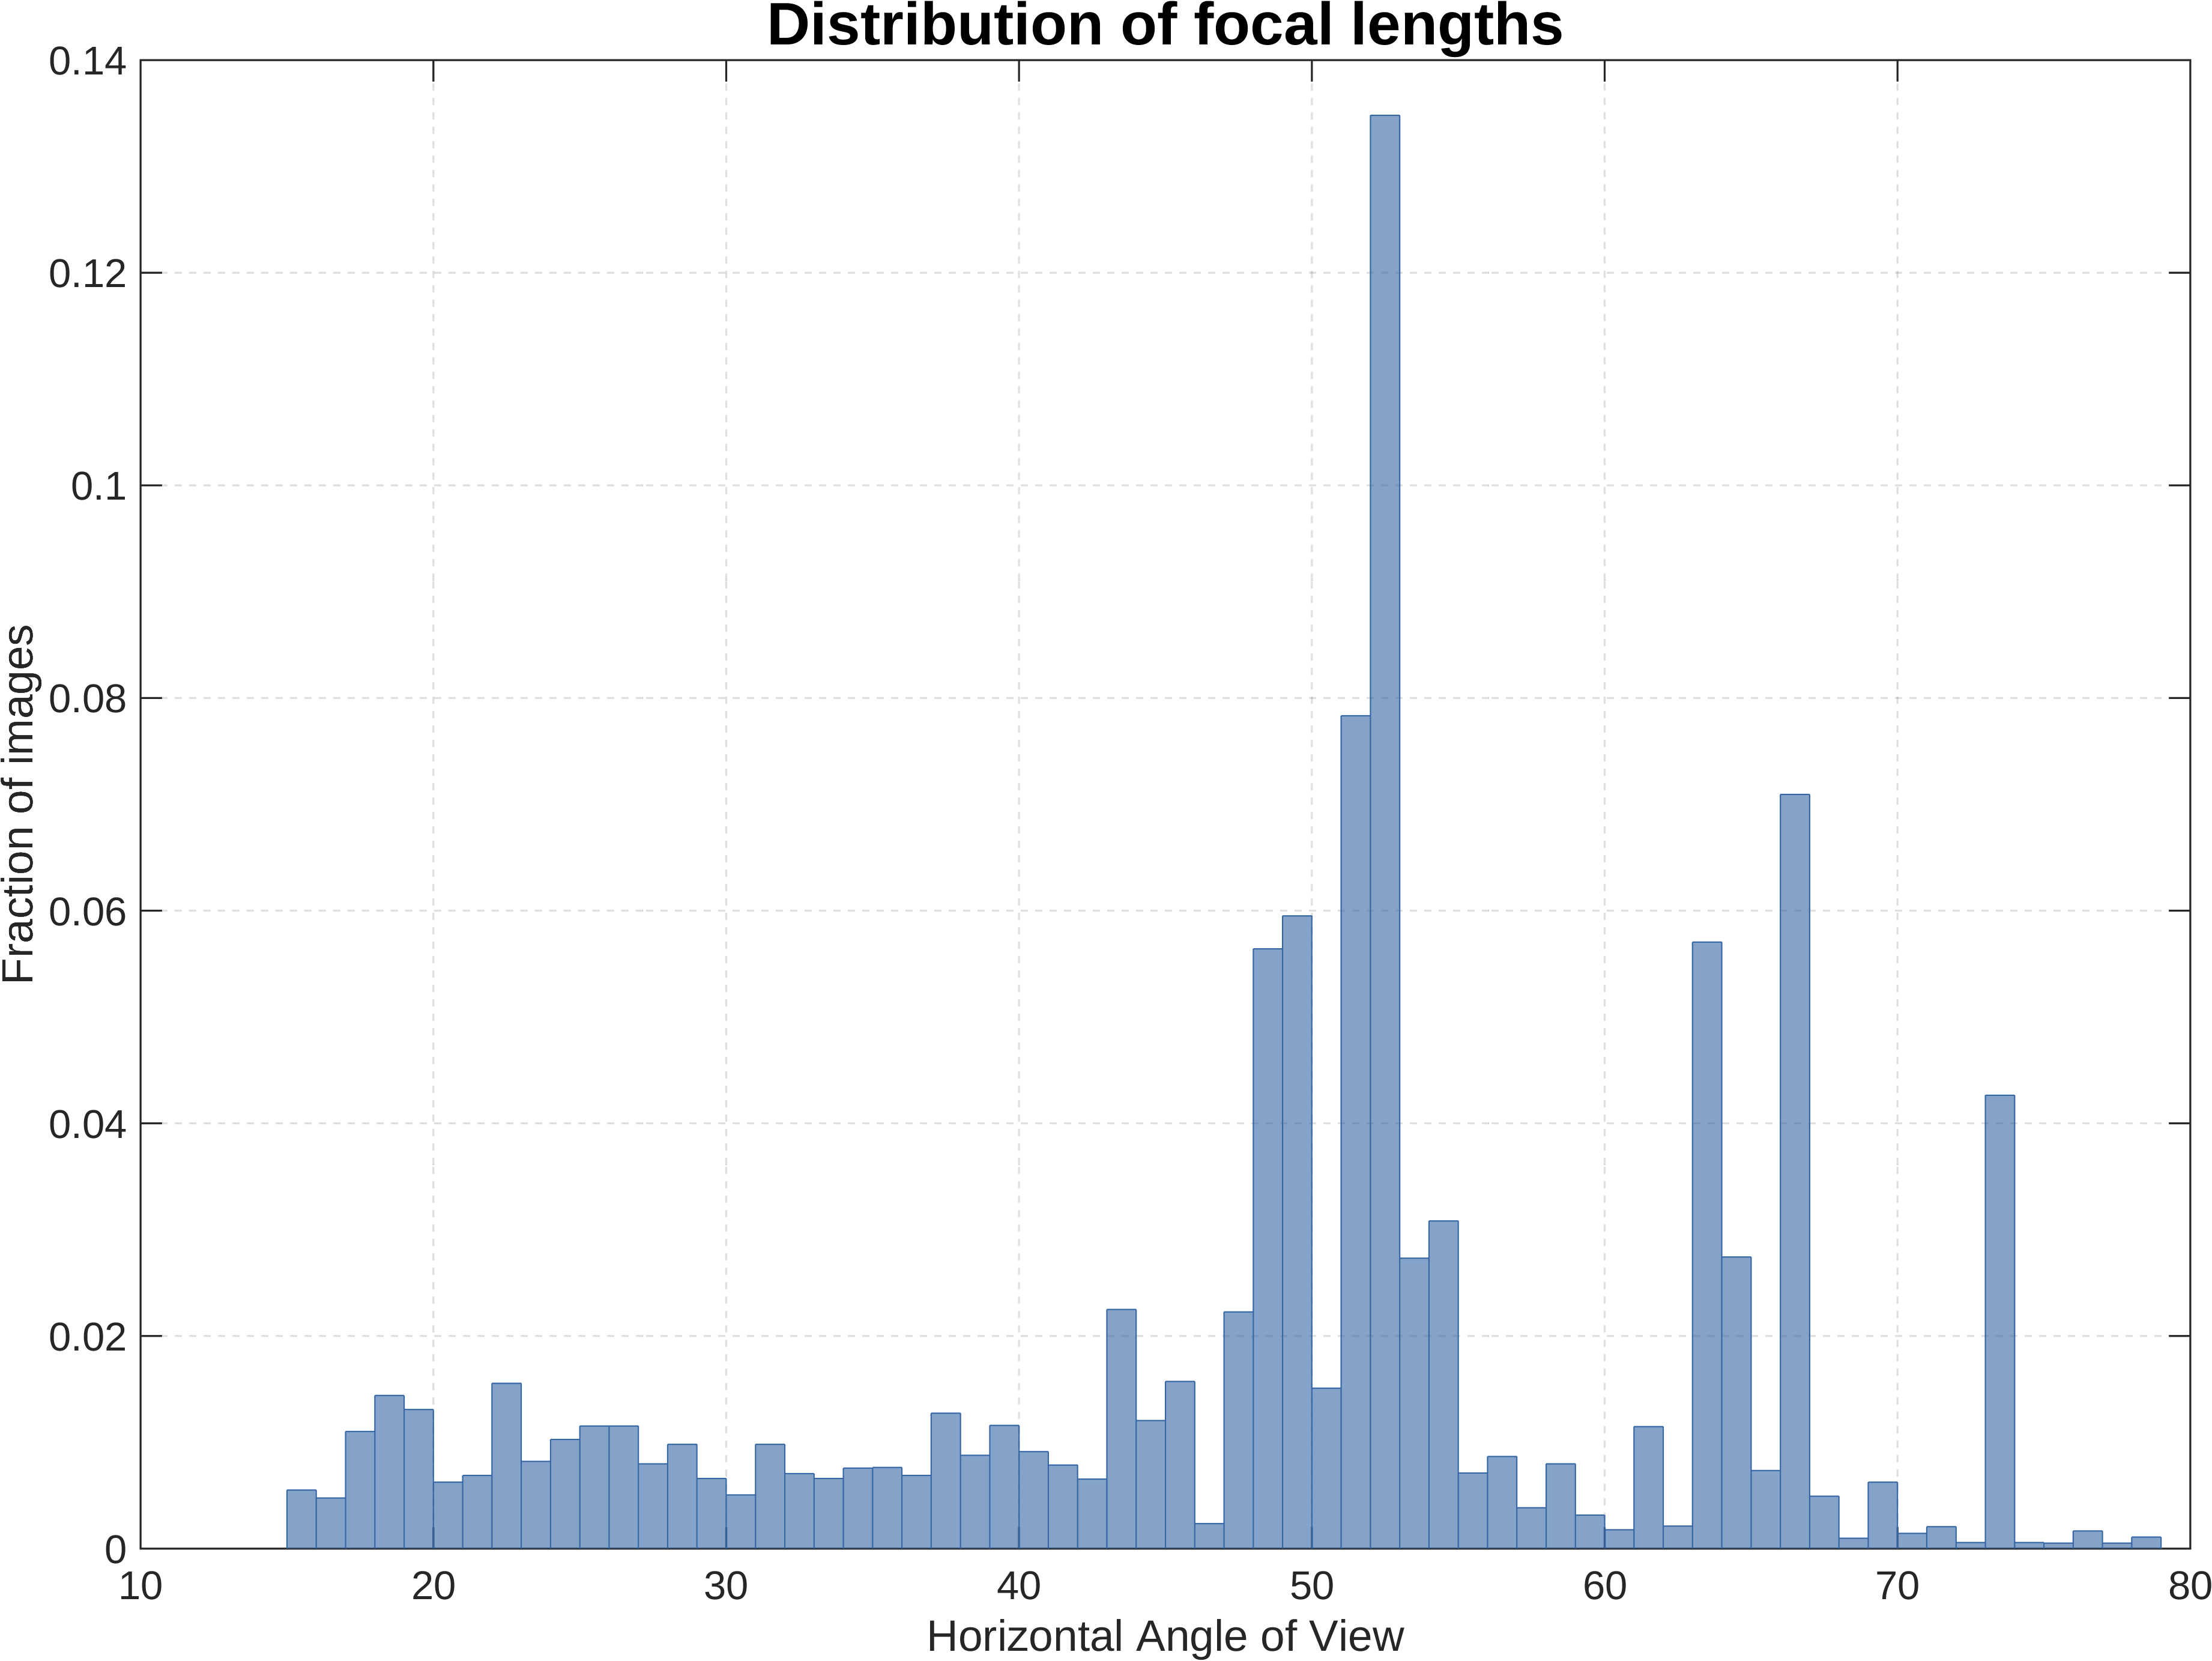
\includegraphics[width=0.95\linewidth]{figures/amodal/fov.png}
    \caption{\figlabel{fovDistr} Distribution of camera focal lengths in the Places dataset shown as horizontal angle of view. The peaks in the distribution correspond to canonical focal lengths in popular wide angle and telephoto lenses. It can be seen that the images cover the full spectrum from wide angle views of scenes (corresponding to the right end of the plot) to close-ups (left end of the histogram).}
  \end{minipage}
  \end{figure}

\paragraph{Results:} The results are shown in \tableref{focal_results} and suggest that focal length can indeed be predicted directly from images, at least approximately, and that pretraining on annotated scene class data makes a good match with this task. Our best model can predict correct focal length quite repeatably  among the top-three and top-five predictions. As baselines, we measure chance performance, and performance when picking the mode of the distribution on the training set -- the bin having most elements. The (unequal) distribution of the focal lengths can be seen in \figref{fovDistr}.


Note that our goal is not high precision of the type that is necessary for high-fidelity reconstruction; we aim for a coarse estimate of the focal length that can be robustly computed from natural images. Our results in this section are a first demonstration that this may be feasible.

\begin{table}
\centering
\resizebox{0.5\linewidth}{!}{
 \begin{tabular}{ l  c  c c}
\toprule
\textbf{Method} & \textbf{top-1} & \textbf{top-3} & \textbf{top-5} \\
\midrule
Chance & 90.0 & 70.0 & 50.0 \\
Mode Selection & 60.2 & 26.4 & 8.7 \\
\midrule
AlexNet-Imagenet & 57.1  & 18.8 & 3.9 \\
VGG-Deep16-Imagenet & 55.8 & 15.9 & 3.3 \\
PlacesNet-Places & \textbf{54.3} & \textbf{15.3} & \textbf{3.1} \\
\bottomrule
  \end{tabular}}
    \caption{\tablelabel{focal_results}Focal length misclassification rate (top-1, top-3 and top-5 predictions) of networks pretrained on object images from Imagenet and the Places dataset. Lower is better.}
\end{table}